\documentclass[a4paper]{article}
\usepackage[utf8]{inputenc}
\usepackage{graphicx}

\begin{document}

\section{Vererbung}

Gregor Mendel (1822 - 1884) war zuständig für den Klostergarten (Mönch). Er hat zufällig Erbsen in verschiedenen Farben gepflanzt. Er hat nun verschiedene Farben miteinander gekreuzt, um zu sehen was passiert.
\newline
\newline
Unformitätsregel:
\newline
\newline
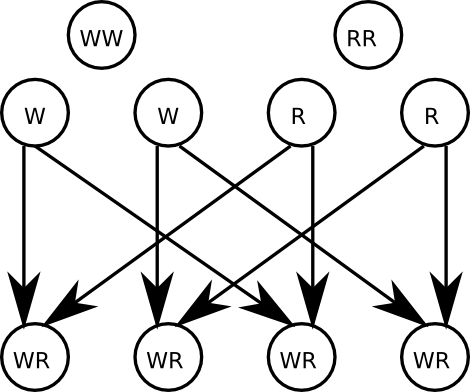
\includegraphics[scale=0.25]{image/1.png}
\newline
\newline
Spaltungsregel:
\newline
\newline
Tritt bei reinrassigen Eltern sind in der ersten Generation alle Kinder Mischlinge. Genotypus sind alle gespeicherten Merkmalen in der Zelle. Phenotypus sind alle ausgebildeten Merkmale. Merkmale können rezessiv oder dominat sein. Dominante Merkmale setzten sich bei Kreuzungen mit rezessiven Merkmale durch und werden ausgebildet. Die Körperzelle hat alle Merkmale doppelt gespeichert (nennt man Diploid). Die Geschlechtszellen haben die Merkmale nur einmal gespeichert (nennt man Happloid).
\newline
\newline
Die Bluterdkrankheit können sich bei Inzucht besonders gut weiterbilden. Der Mann erkrankt jedoch leichter als die Frau, da Männer (XY Chromosom) schon erkrankt sind wenn das X die Krankheit hat. Bei der Frau (XX Chromosom) müssen beide X-Chromosome erkrankt sein, damit die Frau die Krankheit hat.

\newpage

\section{Zellteilung}

Die Zellteilung wird auch Mitose genannt (normale Körperzellteilung). Zellen enstehen nur durch die Zellteilung.

\subsection{DNS - Desoxyribonukleinsäure}

Die DNS kann sich vervielfältigen, denn bevor die Zellteilung beginnt muss sich die DNS mit den Erbinformationen kopieren. 

Aufbau der DNS:

Die DNS ist besteht aus einen Doppelstrang und jeder Strang besteht aus Tripplets. Ein Tripplet sind drei Basen. Viele Tripplets bilden eine Aminosäure (=Eiweiß). Viele Eiweiße sind ein Gen und viele Gene ist ein Chromosom und viele Chromosome bilden die DNA.

Bei der Zellteilung muss die DNS vollständig kopiert werden, dabei öffnet sich der Doppelstrang und durch Anlieferung und Ablagerung entsprechender Basen werden aus einem Doppelstrang zwei Doppelstränge $\rightarrow$ entspricht der identen Kopie der Chromosomen. Eine plötzlich spontane Änderung der Erbinformation durch Kopierfehler oder anderen Ursachen (Energiereiche Strahlung, Chemikalien) nennt man Mutation (99,99\% alle Mutationen sind negativ behaftet, die positiven Mutationen sind mit Triebfehler für die Evolution behaftet).

\newpage

\section{Makromoleküle}

\subsection{Kohlenhydrate}

\subsection{Eiweiße (=Proteine)}

\subsection{Fette}

\newpage

\section{Gesundheit}

Richtige Ernährung

Ernährung heißt Energie zuführen. 
Energie kann auf verschiedene Form - in chemischer Form zugeführt werden
die Stoffe haben einen bestimmten Joule Wert 1k Kalorie = 4,2k Joule

Jetzt ist es so das man als ausgeachsenen mensc einen bestimmten joule verbraucht. weil es den betriebswert gi bt endoterm es muss energie zugeührt werden zusätlich kommt ein teil dazu wenn man aktiv ist (bewegung) 

Der Grundbedarf ist der Bedarf an Energie, die ein Mensch beim Sitzen oder Liegen verbraucht. Der Grundumsatz (=Grundbedarf) bei einem 70 Kilo Menschen ist in etwa 7000k Joule. Tätigkeitsumsatz kann bis zu 20000k Joule zusätzlich brauchen.

Der Mensch ist ein Heterotropher, der Mensch ist ein Allesfresser. Der Fettanteil sollte 25\% der Eingenommen Essen (hängt vom Verbrauch aus). Vitamine sind Stoffe, die der Körper nicht alleine herstellen kann.

Wichtige Vitamine:

\begin{itemize}
\item Vitamin A (Retinol)
\item Vitamin B1 (Thiamin)
\item Vitamin B2-Gruppe 
\item Vitamin B6 (Pyridxoin)
\item Vitamin B12 (Cobalamin)
\item Vitamin C
\item Vitamin D

\item Vitamin E (Fruchtbarkeisvitamin)
\item Vitamin K (
\end{itemize}


\end{document}